\documentclass[12pt]{article} 
\usepackage[utf8]{inputenc}
\usepackage{geometry}
\geometry{letterpaper}
\usepackage{graphicx} 
\usepackage{parskip}
\usepackage{booktabs}
\usepackage{array} 
\usepackage{paralist} 
\usepackage{verbatim}
\usepackage{subfig}
\usepackage{fancyhdr}
\usepackage{sectsty}
\usepackage{bbm}
\usepackage[shortlabels]{enumitem}

\pagestyle{fancy}
\renewcommand{\headrulewidth}{0pt} 
\lhead{}\chead{}\rhead{}
\lfoot{}\cfoot{\thepage}\rfoot{}


%%% ToC (table of contents) APPEARANCE
\usepackage[nottoc,notlof,notlot]{tocbibind} 
\usepackage[titles,subfigure]{tocloft}
\renewcommand{\cftsecfont}{\rmfamily\mdseries\upshape}
\renewcommand{\cftsecpagefont}{\rmfamily\mdseries\upshape} %

\usepackage{amsmath}
\usepackage{amssymb}
\usepackage{mathtools}
\usepackage{empheq}
\usepackage{xcolor}

\usepackage{tikz}
\usepackage{pgfplots}
\usepackage{tikz-cd}
\usepackage{tikz-qtree}
\pgfplotsset{compat=1.18}

\newcommand{\ans}[1]{\boxed{\text{#1}}}
\newcommand{\vecs}[1]{\langle #1\rangle}
\renewcommand{\hat}[1]{\widehat{#1}}
\newcommand{\F}[1]{\mathcal{F}(#1)}
\renewcommand{\P}{\mathbb{P}}
\newcommand{\R}{\mathbb{R}}
\newcommand{\E}{\mathbb{E}}
\newcommand{\Z}{\mathbb{Z}}
\newcommand{\N}{\mathbb{N}}
\newcommand{\Q}{\mathbb{Q}}
\newcommand{\ind}{\mathbbm{1}}
\newcommand{\qed}{\quad \blacksquare}
\newcommand{\brak}[1]{\left\langle #1 \right\rangle}
\newcommand{\bra}[1]{\left\langle #1 \right\vert}
\newcommand{\ket}[1]{\left\vert #1 \right\rangle}
\newcommand{\abs}[1]{\left\vert #1 \right\vert}
\newcommand{\mfX}{\mathfrak{X}}
\newcommand{\ep}{\varepsilon}

\newcommand{\sub}{\subseteq}

\usepackage{tcolorbox}
\tcbuselibrary{breakable, skins}
\tcbset{enhanced}
\newenvironment*{tbox}[2][gray]{
    \begin{tcolorbox}[
        parbox=false,
        colback=#1!5!white,
        colframe=#1!75!black,
        breakable,
        title={#2}
    ]}
    {\end{tcolorbox}}

    

\title{APMA 1930X: Probability, Optimization, and Stochastic Calculus}
\author{Milan Capoor}
\date{Fall 2024}

\begin{document}
\maketitle
\section*{Sept 04}
\subsection*{Kelly Betting}
    Imagine a game where 
    \[\begin{tikzcd}
        & 0.90 = 1.9\\ 
        1 \arrow[ur, "50\%"] \arrow[dr, "50\%"]&\\
        & -0.5 = 0.5
    \end{tikzcd}\]  

    So our expected payoff is 
    \[\E(\text{payoff}) = 0.5\cdot 0.9 + 0.5 \times (-0.5) = 0.2\]
    so the game is favorable to you. 

    Now consider the game 
    \[\begin{tikzcd}
        & 0.90x = 1.9x\\ 
        x \arrow["50\%"]{ur} \arrow["50\%"]{dr} &\\
        & -0.5x = 0.5x
    \end{tikzcd}\] 

    The expected payoff is
    \[\E[\text{payoff}] = 0.2x\]
    which is decidedly unfavorable. 

    Now betting all-in is not a good idea. Suppose your current wealth is $S_0$ and wealth after one bet is $S_1$ Consider the log of the second scenario:
    \[\begin{tikzcd}
        & \log(1.9 S_0) = \log(1.9) + \log(S_0)\\ 
        \log S_1 \arrow["50\%"]{ur} \arrow["50\%"]{dr}  &\\
        &  \log(0.5 S_0) = \log(0.5) + \log(S_0)
    \end{tikzcd}\]
    so 
    \[\begin{tikzcd}
        & \log(1.9)\\ 
        \log \frac{S_1}{S_0} \arrow["50\%"]{ur} \arrow["50\%"]{dr}  &\\
        &  \log(0.5 S_0) = \log(0.5)
    \end{tikzcd}\]

    Which tells us that after $n$ bets  
    \[\begin{tikzcd}
        & \log(1.9)\\ 
        \log \frac{S_n}{S_{n-1}} \arrow["50\%"]{ur} \arrow["50\%"]{dr}  &\\
        & \log(0.5)
    \end{tikzcd}\]

    Suppose that each bet is iid with $x_i = \log \frac{s_i}{s_{i-1}}$with $p(x_i = \log 0.5) = 0.5$and $p(x_i = \log 1.9) = 0.5$ Then 
    \[\log \frac{S_n}{S_{n-1}} + \log \frac{S_n-1}{S_{n-2}} + \cdots + \log \frac{S_1}{S_{0}} = X_n + X_{n-1} + \cdots + X_1\]
    hence 
    \[\log S_n = \log S_0 + (X_1 + \cdots + X_n)\] 
    By LLN 
    \begin{align*}
        \lim_{n \to \infty} \frac{1}{n} \sum_i x_i &= \E[X_1]\\ 
        &= 0.5 \log 1.9 + 0.5 \log 0.5\\
        &= 0.5 \log(0.95) < 0 
    \end{align*}
    so $S_n \to 0$ Clearly, all-in betting is not a good idea. 

    What if we bet a very small fraction of our wealth? By LLN, we will \emph{eventually} realize our edge but we will have to wait a long time. Can we do better?

    Now bet $wx$where $0 \leq w \leq 1$ Then 
    \[\begin{tikzcd}
        & x + 0.90wx\\ 
        x \arrow["50\%"]{ur} \arrow["50\%"]{dr} &\\
        & x - 0.5wx
    \end{tikzcd} \implies \begin{tikzcd}
        & \log(1 + 0.9w)\\
        \log \frac{S_n}{S_{n-1}} \arrow["50\%"]{ur} \arrow["50\%"]{dr} &\\
        & \log(1 - 0.5w)
    \end{tikzcd}\]
    so 
    \[\E[\log \frac{S_n}{S_{n-1}}] = 0.5 \log(1 + 0.9w) + 0.5(\log 1 - 0.5w)\] 
    which we want to maximize for $w \in [0, 1]$

    Taking the derivative, we get 
    \[\frac{0.9}{1  +0.9w} - \frac{0.5}{1 - 0.5w} = 0 \implies 0.9 - 0.45w = 0.5 + 0.45w\]
    so the best betting fraction is $w^* = \frac{4}{9}$and 
    \[\E(\log \frac{S_n}{S_{n-1}}) = 0.5\log \frac{9.8}{9} \approx 0.05\]

    We can graph our expected value function 

    \begin{center}
        \begin{tikzpicture}
            \begin{axis}[
                axis lines = middle,
                xlabel = $w$,
                domain=0:1,
                samples=100,
                ymin=-0.25, ymax=0.25,
            ]
            \addplot[
                blue,
                thick
            ]
                {0.5*ln(1 + 0.9*x) + 0.5*ln(1 - 0.5*x)};
            \addplot[red, thick, dotted, label=$w^*$]
                coordinates {(4/9, 0) (4/9, 0.05)};
            \node at (axis cs:4/9, 0.06) [anchor=west, red] {$w^*$};
            \end{axis}
        \end{tikzpicture}
    \end{center}

\subsection*{Probability Review}
    \textbf{Example:} Toss a fair coin $p(H) = p(T) = 0.5$n times. 

    What is the probability of getting an even number of heads? 

    One method is to argue by partitioning the sample space. 

    Alternatively, we can argue from the first toss: Let $x_n = p(\text{even \# of H after n tosses})$ Then after the first toss, 
    \begin{itemize}
        \item if we got heads: we need an odd number of heads in the next $n-1$tosses which happens with probability $1 - x_{n-1}$
        \item if we got tails: we need an even number of heads in the next $n-1$tosses which happens with probability $x_{n-1}$
    \end{itemize}

    Therefore, by the Law of Total Probability, 
    \[x_n = 0.5(1 + x_{n-1}) + 0.5(x_{n-1}) = 0.5\]
    
    We call this method \textbf{First step analysis}

\section{Sept 06}
    Last time we ended with an example of a fair coin tossed $n$times. How can we compute 
    \[x_n = P(\text{even \# H with n tosses})\]

    \textbf{Method 1:} Make a partitioning argument, taking advantage of the equal probabilities of heads and tails.

    \textbf{Method 2:} First step analysis.
    
    We argue that on the first toss, if we get heads, then the final probability we have an even number of heads is the same as the probability we have an odd number of heads after $n-1$tosses. If we get tails, then the probability we have an even number of heads is the same as the probability we have an even number of heads after $n-1$tosses.

    Using the law of total probability, we get
    \[x_n = \frac{1}{2}(1 - x_{n-1}) + \frac{1}{2}x_{n-1} = \frac{1}{2}\]

    \textbf{The Law of Total Probability:} 
    Consider the example 
    \[\begin{tikzcd}
        & E \arrow[r] &  P(B \; | \; E)\\
        \cdot \arrow[ur, "P(E)"] \arrow[dr, "P(E^c)"] \\
        & E^c \arrow[r] & P(B \; | \; E^c)
    \end{tikzcd}\]

    Then 
    \begin{tbox}{\textbf{Law of total Probability:}
        \[P(B) = P(E) P(B \; | \; E) + P(E^c)P(B \; | \; E^c)\]}
        \emph{Proof:} 
        \begin{align*}
            RHS &= P(E)P(B \; | \; E) + P(E^c)P(B \; | \; E^c)\\
            &= P(E)\frac{P(B \cap E)}{P(E)} + P(E^c)\frac{P(B \cap E^c)}{P(E^c)}\\
            &= P(B \cap E) + P(B \cap E^c)\\
            &= P(B)\\ 
            &= LHS
        \end{align*}
    \end{tbox}

    Consider a scenario with a biased coin with $p(H) = p$ and $p(T) = q$ Now 
    \begin{align*}
        x_n &= p(1 - x_{n-1}) + qx_{n-1}\\ 
        &= p + (q - p)x_{n-1}
    \end{align*}

    We want a special solution to this equation which is a constant in $n$, i.e. $x_n = c$ 

    We know $x_1 = P(T) = q$ 

    Start with the guess $c = \frac{1}{2}$ Then 
    \begin{align*}
        x_n &= p + (1 - 2p)x_{n-1}\\
        x_n - \frac{1}{2} &= p + (1 - 2p)x_{n-1} - \frac{1}{2}\\ 
        &= (1 - 2p)(x_{n-1} - \frac{1}{2})\\ 
        &= (1 - 2p)(1 - 2p)(x_{n-2} - \frac{1}{2})\\ 
        &= \cdots\\
        &= (1 - 2p)^{n-1}(x_1 - \frac{1}{2})\\
        &= (1 - 2p)^{n-1}(p - \frac{1}{2})
    \end{align*}
    so 
    \[\boxed{x_n = \frac{1}{2} + (1 - 2p)^{n-1}(q - \frac{1}{2}) = \frac{1}{2} + \frac{1}{2}(1 - 2p)^n}\]

    Thus, we can say the general method is 1) use first-step analysis to get a recursive formula and 2) guess a solution and prove it by induction.

    \textbf{Example (Putnam 2001):} We have $n$coins $C_1, C_2, \ldots, C_n$with $P(C_k = H) = \frac{1}{2k + 1}$ What is the probability that the number of heads is odd after tossing all $n$coins?

    Let's try the same approach as last time.

    Let $x_n = P(\text{odd \# of heads after n coins})$ Then the first toss gives us 
    \[x_1 = P(C_1 = H) = \frac{1}{3}\]
    \[\begin{tikzcd}
        & H\\
        C_{1} \arrow[ur, "\frac{1}{3}"] \arrow[dr, "\frac{2}{3}"] &\\
        & T 
    \end{tikzcd}\]
    But in fact this tells us nothing because the probability of getting an even number of heads in the next $n-1$ tosses is not $1 - x_{n-1}$ but some function of $\frac{1}{2k+1}$ 

    We actually need to start from the last toss:
    \[\begin{tikzcd}
        & H \arrow[r, dashed, no head] & 1 - x_{n-1} \quad \text{(even \# H in first (n-1) tosses)}\\ 
        x_{n} \arrow[ur, "{\frac{1}{2n+1}}"] \arrow[dr, "{\frac{2n}{2n+1}}"] &\\
        & T \arrow[r, dashed, no head] & x_{n-1} \quad \text{(odd \# H in first (n-1) tosses)}
    \end{tikzcd}\]

    So 
    \begin{align*}
        x_n &= \frac{1}{2n+1}(1 - x_{n-1}) + \frac{2n}{2n+1}x_{n-1}\\
        &= \frac{1}{2n+1} + \frac{2n - 1}{2n+1}x_{n-1}
    \end{align*}

    Again guessing $x_n = \frac{1}{2}$, 
    \begin{align*}
        x_n - \frac{1}{2} &= \frac{2n - 1}{2n + 1}(x_{n-1} - \frac{1}{2})\\ 
        &= \frac{2n - 1}{2n + 1}\frac{2n - 3}{2n - 1}(x_{n-2} - \frac{1}{2})\\
        &= \frac{2n - 1}{2n + 1}\frac{2n - 3}{2n - 1}\cdots \frac{3}{5}(x_{1} - \frac{1}{2})
        &= \cdots\\
        &= \frac{3}{2n+1}(\frac{1}{3}- \frac{1}{2})\\ 
        &= -\frac{1}{2(2n+1)}\\
        x_n &= \frac{1}{2} - \frac{1}{2(2n+1)} = \boxed{\frac{n}{2n + 1}}
    \end{align*}

    \textbf{Example (Law of Total Probability for Continuous RV)}: When we have finitely many possible outcomes, we can simply sum them by the LTP. What if we have infinitely many? 
    
    Consider a coin where $P(H) \sim \text{Unif}[0, 1]$ If we toss the coin $n$ times and define $X = $ \# of H, what is $P(X = k), k = 0, 1, \dots, n$?

    (Easier variation) Define $\theta = P(H) \sim \text{Unif}[0, 1]$ Suppose we are given $\theta = p$ Now 
    \[P(X = k \; | \; \theta = p) = \binom{n}{k} p^k (1 -p)^{n-k}\]

    For the continuous case, we have 
    \[P(X = k) = \int_0^1 P(X = k \; | \; \theta = p) \cdot (\text{density of } \theta \text{ at } p)\; dp\]

    But the density of $\theta$ at $p$ is simply 1 (uniform!). So
    \[P(X = k) = \int_0^1 \binom{n}{k} p^k (1 - p)^{n-k} \; dp\]
    
    Let's do some examples:
    \[P(X = 0) = \int_0^1 (1 - p)^n \; dp = \frac{1}{n + 1}\]
    (hint: change of variables $u = 1 - p$)

    \begin{align*}
        P(X = 1) &= \int_0^1 n p(1-p)^{n-1} \; dp\\ 
        &\overset{x = 1 - p}{=} \int_1^0 n(1 - x)x^{n1}\; (-dx)\\ 
        &= \int_0^1 nx^{n-1} - nx^n\; dx\\ 
        &= 1  - n \frac{1}{n + 1} = \frac{1}{n + 1}
    \end{align*}

    \begin{align*}
        P(X = n) = \int_0^1 p^n \; dp = \frac{1}{n + 1}
    \end{align*}

    So we conclude $P(X = k) = \frac{1}{n + 1}$

\section{Sept 09}
    Last time we introduced the \emph{continuous version of the Law of Total Probability}:
    \[P(A) = \int P(A \; | \; X = x) f_X(x)\; dx\]

    \textbf{Example:} Suppose you have a fair die ($X \in 1...6$). 
    \begin{enumerate}
        \item What is the average number of tosses until 6 appears?
        \item What is the average cumulative sum ($\sum x_i$) until 6 appears?
    \end{enumerate}

    Every time we toss the die, we know $P(6) = \frac{1}{6}$ and $P(\lnot 6) = \frac{5}{6}$. If $X$ is the number of tosses until 6, we know 
    \[X \sim \text{geometric}(p) \implies \E[X] = \frac{1}{p}\]

    Which we can see from 
    \begin{align*}
        \E[X] &= \sum_{i=1}^n P(X = n) \cdot n\\ 
        &= \sum_{i=1}^n (1- p)^{n-1} p \cdot n\\ 
        &\vdots\\ 
        &= \frac{1}{p}
    \end{align*}

    This method presents some difficulties in general: How do we explicitly know $P(X = n)$. Further, this method tells us nothing about question 2. 

    Let's try again with FSA: Let $X$ be the average number of tosses until 6. 

    Look at the first toss:

    \begin{center}
        \begin{tabular}{|p{1in}p{1in}|}
            \hline\\
            \multicolumn{2}{c}{1st Toss}\\ 
            Outcome on first toss & Average number of tosses to reach 6\\ 
            \hline
            1 & $x$\\ 
            2 & $x$\\ 
            3 & $x$\\ 
            4 & $x$\\ 
            5 & $x$\\ 
            6 & $0$\\ 
            \hline
        \end{tabular}
    \end{center}
   

    So 
    \[X = 1 + \frac{5}{6}x + \frac{1}{6}\cdot 0 = 1 + \frac{5}{6}X \implies \boxed{X = 6}\] 
    (the $1$ is the first toss we already used) 

    Now let $Y$ be the average cumulative sum until 6. We can draw exactly the same table because for each case the average depends on all the rest: 
    
    \begin{center}
        \begin{tabular}{|p{1in}p{1in}|}
            \hline\\
            \multicolumn{2}{c}{1st Toss}\\ 
            Outcome on first toss & Average number of tosses to reach 6\\ 
            \hline
            1 & Y\\ 
            2 & Y \\ 
            3 & Y\\ 
            4 & Y\\ 
            5 & Y\\ 
            6 & 0\\ 
            \hline
        \end{tabular}
    \end{center}
    
    so 
    \begin{align*}
        Y &= \frac{1}{6}(1 + y) + \frac{1}{6}(2 + y) + \cdots + \frac{1}{6}(5 + y) + \frac{1}{6}(6 + 0)\\ 
        &= \frac{5}{6}y + \frac{7}{2}\\ 
        &= 21
    \end{align*}

    \textbf{Example:} Toss a coin $n$ times and let $P(H) = p$. What is the probability that the pattern $HH$ does not appear? 

    Let $x_n$ be the probability that $HH$ does not appear after $n$ tosses. Then we know 
    \begin{align*}
        x_1 &= 0\\ 
        x_2 &= 1 - p^2
    \end{align*}
    but the rest become very complicated. 

    For simplicity, let $P(T) = q = 1 - p$.

    \begin{center}
        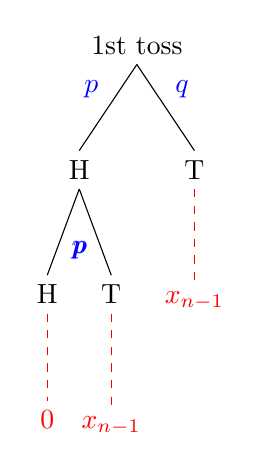
\begin{tikzpicture}[level distance=45]
            \Tree [.{1st toss} 
                    \edge node[auto=right, blue]{$p$}; [.H
                        \edge node[auto=left, blue]{$p$}; [.H \edge[dashed, red, auto=right]; \node[red]{0};] 
                        \edge node[auto=right, blue]{$p$}; [.T \edge[dashed, red, auto=right]; \node[red]{$x_{n-1}$};]]
                    \edge node[auto=left, blue]{$q$}; [.T \edge[dashed, red, auto=right]; \node[red]{$x_{n-1}$};]
                ]
        \end{tikzpicture}
    \end{center}

    So 
    \[x_n = qx_{n-1} + pqx_{n-2}, \quad x_1 = 1, x_2 = 1 - p^2\]

    We can solve this using a method similar to 2nd order ODEs: 
    \[f'' + af' + bf =0 \implies r^2 + ar + b = 0 \implies f = C_1e^{r_1 t} + C_2e{r_2 t}\]

    In our case 
    \[x_n = qx_{n-1} + pqx_{n-1} \implies r^2 = qr + pq\]

    We can find roots $r_1, r_2$ and then solve for $C_1, C_2$ using the initial conditions, giving our solution:
    \[\begin{cases}
        x_n = Ar_1^n + Br_2^n\\ 
        x_1 = 1, \; x_2 = 1- p^2
    \end{cases}\]

    \textbf{Example:} We are playing a game of dice with the following rules:

    \begin{enumerate}
        \item If the toss is 1, 2, 3, you get the face value and continue 
        \item If the toss is 4, 5, you get the face value and the game ends
        \item If the toss is 6, the game ends 
    \end{enumerate}

    \emph{Example game:} $3 \to 2 \to 2 \to 4$ gives score $11$

    What is the average payoff $x$? 
    \begin{center}
        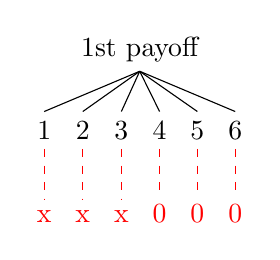
\begin{tikzpicture}
            \Tree [.{1st payoff}
                [.1 \edge[red, dashed]; \node[red]{x};] 
                [.2 \edge[red, dashed]; \node[red]{x};] 
                [.3 \edge[red, dashed]; \node[red]{x};] 
                [.4 \edge[red, dashed]; \node[red]{0};]
                [.5 \edge[red, dashed]; \node[red]{0};] 
                [.6 \edge[red, dashed]; \node[red]{0};]]
        \end{tikzpicture}
    \end{center}

    So 
    \[x = \frac{1}{6}(1 + x) + \frac{1}{6}(2 + x) + \frac{1}{6}(3 + x) + \frac{1}{6}(4 + 0) + \frac{1}{6}(5 + 0) + \frac{1}{6}(0) = 5\]

\section{Sept 11}
    \textbf{Harder Variation:} now the game rules are 
    \begin{enumerate}
        \item If the toss is 1, 2, 3, you get the face value and continue 
        \item If the toss is 4, 5, you get the face value and the game ends
        \item If the toss is 6, the game ends and you lose all your points
        \item You can stop the game whenever you want 
    \end{enumerate}

    Let $y$ be the average cumulative sum. Now 

    \begin{center}
        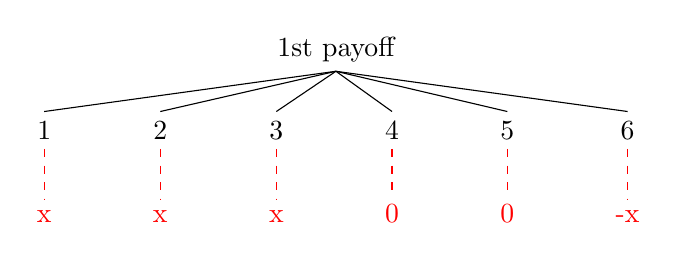
\begin{tikzpicture}[sibling distance=30pt]
            \Tree [.{1st payoff}
                [.1 \edge[red, dashed]; \node[red]{x};] 
                [.2 \edge[red, dashed]; \node[red]{x};] 
                [.3 \edge[red, dashed]; \node[red]{x};] 
                [.4 \edge[red, dashed]; \node[red]{0};]
                [.5 \edge[red, dashed]; \node[red]{0};] 
                [.6 \edge[red, dashed]; \node[red]{-x};]]
        \end{tikzpicture}
    \end{center}

    Recall that in the previous case where the game ended on 6 but you retained your score, 
    \[x = \frac{1}{6}(1 + x) + \frac{1}{6}(2 + x) + \frac{1}{6}(3 + x) + \frac{1}{6}(4 + 0) + \frac{1}{6}(5 + 0) + \frac{1}{6}(0) = 5\]

    However, in the new game this is not quite right: we are not guaranteed to keep our early points if we continue. What is the probability we keep our points? $2/3$ because out of the three ending conditions, we keep our points in two of them.

    So 
    \[y = \frac{1}{6}(\frac{2}{3} + y) + \frac{1}{6}(\frac{4}{3} + y) + \frac{1}{6}(2 + y) + \frac{1}{6}(4) + \frac{1}{6}(5) \implies \boxed{y = \frac{13}{3}}\]

    But this really only works because the stopping condition is simple. 

    \textbf{Example (Prison Dilemma):} 100 prisoners are given a chance to play a game for their freedom. There are 100 boxes that each contain a paper with a number from 1 to 100. Each prisoner has a number 1-100 and is allowed to open 50 boxes. If one of these 50 boxes contain his number, he wins. If all 100 prisoners win, they all go free. If anybody loses, they are all executed. 

    We know that if each prisoner opens boxes at random, the probability of winning is $\frac{1}{2^{100}}$. Can they do better?

    Here is one strategy, though we can't say if it is optimal: 
    \begin{enumerate}
        \item Each player opens the box corresponding to their number
        \item If they don't win, they open the box corresponding to the number on the paper in the box they just opened
        \item Repeat until they win or they have opened 50 boxes
    \end{enumerate}

    We are looking for cycles in the graph. If the cycle has length at most 50, everyone in the cycle wins. If the cycle is longer than 50, everyone loses.
    
    As cycles are disjoint, we can partition the space. Then everyone will win if all the cycles are of length at most 50 so 
    \begin{align*}
        \P(\text{win}) &= \P(\text{every cycle } \leq 50)\\
        &= 1 - \P(\text{at least one cycle} > 50)\\ 
        &= 1 - \P(\text{exactly one cycle} > 50)
    \end{align*}

    Let's look more generally: for $2n$ boxes what is the probability one cycle is of length at least $n$?
    \[\P(\text{one cycle } > n) = \sum_{k={n+1}}^{2n} \P(\text{one cycle} = k)\]

    We can view the contents of the boxes in order as a permutation of $2n$ elements. We know there are $(2n)!$ permutations. How many give a cycle of length $k$?

    Clearly, we want to choose $k$ elements to be in the cycle and then permute the rest. So
    \[\binom{2n}{k}(2n - k)!\]
    But how many ways are there to make a cycle with $\binom{2n}{k}$ elements? $(k-1)!$ 

    All togehter, 
    \begin{align*}
        \P(\text{one cycle} = k) &= \frac{1}{(2n)!} \binom{2n}{k}(2n - k)!(k-1)!\\ 
        &= \frac{1}{(2n)!}\frac{(2n)!}{(2n -k)!k!} (2n-k)!(k-1)!\\ 
        &= \frac{(k-1)!}{k!}
    \end{align*}

    So 
    \[\P(\text{win}) = 1 - \sum_{k=n+1}^{2n} \frac{1}{k}\]

    We can approximate 
    \[1 + \frac{1}{2} + \frac{1}{3} + \cdots + \frac{1}{n} = \log n + C\]
    for a constant $C$ so 
    \begin{align*}
        \P(\text{win}) &= 1 - \sum_{k=n+1}^{2n} \frac{1}{k}\\ 
        &= 1 - \left(\sum_{k=1}^{2n} \frac{1}{k} - \sum{k=1}^n \frac{1}{k}\right)\\ 
        &\approx 1 - (\log 2n + C - (\log n + C))\\ 
        &= 1 - \log 2 \approx 0.3
    \end{align*}

\section{Sept 13:}
\subsection*{Law of Total Expectation}
    \textbf{Example:} In America, 50.5\% of the population is female, 49.5\% is male. The average life expectancy is 79.1 for women and 73.2 for men. What is the average life expectancy of an American?

    \begin{align*}
        \frac{1}{N} \sum_{\text{Americans}} \text{life expectancy} &= \frac{1}{N} \sum_{\text{Women}} \text{life expectancy} + \frac{1}{N} \sum_{\text{Men}} \text{life expectancy}\\
        &= \frac{1}{N}(0.505N \cdot 79.1) + \frac{1}{N}(0.495N \cdot 73.2)\\
        &= 76.2
    \end{align*}
    or, in general, 
    \[P(A) = \sum_y P(A \; | \; Y = y)P(Y = y)\]

    This is incredibly intuitive but let's generalize. Say $Y$ is the average life expectancy of an American and $X$ is their sex. Let $X = 1$ if woman, $X =0$ if man. 
    Then the situation is expressed 
    \[\begin{cases}
        \P(X = 1) = 50.5\%, \quad \P(X = 0) = 49.5\%\\ 
        \E[Y \; | \; X = 1] = 79.1, \quad \E[Y \; | \; X = 0] = 73.2
    \end{cases}\]  


    Therefore, if we define a random variable $\E[Y \; | \; X]$ such that it takes value $\E[Y \; | \; X = 1]$ on event $X = 1$ and $\E[Y \; | \; X = 0]$ on event $X = 0$, then
    \[\E[Y] = \E[Y \; | \; X=1] \P(X = 1) + \E[Y \; | \; X = 0] \P(X = 0) = \E[\E[Y \; | \; X]]\]
    
    For $Y$ discrete, 
    \[\E[Y] = \E[\E[Y \; | \; X]] = \sum_y \E[X \; | \; Y = y] \P(Y = y)\]

    We call $E[Y \; | \; X]$ the \emph{conditional expectation} of $Y$ given $X$. 

    The Law of Total Expectation is a Generalization of the law of total probability. 

    Define for all $A \sub \Omega$, the \emph{indicator random variable} by
    \[\ind_{A}(\omega) = \begin{cases}
        1 & \omega \in A\\
        0 & \omega \notin A
    \end{cases}\]  

    Then, staightforwardly, $\P(A) = \E[\ind_A]$ and the Law of Total Probability is 
    \[\P(A) = \E \; | \; \P(A \; | \; X)\] 
    for any family of random variables $X$. 
    
    When $X$ is a single random variable: 
    \begin{align*}
        \P(A) &= \sum_i \P(A \; | \; X = x_i) \P(X = x_i)\\ 
        \P(A) &= \int_{\R} \P(A \; | \; X= x) f_X(x)\; dx
    \end{align*}
    depending on whether $X$ is discrete or continuous.

    \textbf{Example:} Sample $X_1, X_2, \dots, X_n \sim \text{Unit}[0, 1]$. Let $X_{(1)} = \min \{X_i$\}, $X_{(2)} = \min\{X_i \; | \; X_i \neq X_{(1)}\}$, etc.

    Then $X_{(1)} \leq X_{(2)} \leq \cdots \leq X_{(n)}$ is a rearrangement of $\{X_1, X_2, \dots, X_n\}$ is ascending order, what we call \emph{the order statistics} 

    These $n$ points now partition $[0, 1]$ into $(n+1)$ pieces. What is the average length of each piece? 

    It suffices to find the density of $X_{(1)}$ and compute $\E[X_{(1)}]$ and then compute the average length of each subinterval.

    First, we calculate the CDF:
    \[F_1(x) = \P(X_{(1)} \leq x) = 1 - \P(X_{(1)} > x) = 1 - (1 - x)^n\] 

    Then the density is
    \[f_1(x) = F_1'(x) = n(1-x)^{n-1} \cdot \ind_{[0, 1]}(x)\] 
    and 
    \begin{align*}
        E[X_{(1)}] &= \int_{\R} x f_1(x) \; dx\\ 
            &= \int_0^1 x n(1-x)^{n-1} \; dx\\
            &= \int_0^1 n(1 - t)t^{n-1}\; dt\\ 
            &= \int_0^1 n(t^{n-1} - t^n)\; dt\\ 
            &= 1 - \frac{n}{n+1}\\ 
            &= \frac{1}{n+1}
    \end{align*}

    The first piece on $[0, 1]$ is $[0, X_{(1)}]$ which has average length $\E[X_{(1)}] = \frac{1}{n + 1}$. 

    What about the second piece? 
    \begin{align*}
        \E[X_{(2)}] &= \E[\E[X_{(2)} \; | \; X_{(1)}]] \\ 
        &= \E[\frac{1}{n}(1 - X_{(1)})]\\ 
        &= \frac{1}{n} - \frac{1}{n}\E[X_{(1)}]\\
        &= \frac{1}{n}\left(1 - \frac{1}{n(n+1)}\right)\\
        &= \frac{1}{n+1}
    \end{align*}

    Repeating this procedure, we can see that each interval has average length $\frac{1}{n+1}$

\section{Sept 9}
\subsection*{Optimization}
        \textbf{Classic Optimization:} Given a sequence or function, find its max/min 

        \emph{Method:} Take the derivative and set it equal to zero.

        \textbf{Constrained Optimization:} e.g. maximize $f(x)$ given $g(x) = 0$

        \emph{Method:} Lagrange Multipliers 

        \textbf{Infinite Dimensional Problems:} e.g. $\max_f \, H(f)$ (where $H$ is a function of functions or a \emph{functional})

        \emph{Method:} Calculus of Variations
    
        \textbf{Example (Application of indicator RVs):} A company has $n$ employees. Anyone can take the day off if it is the birthday of some employee. Every work day is 8 hours. How many employees should the company hire so that the total working hour from employees is maximized? 
        
        Denote $a_n = \E[\text{total working hours with } n \text{ employees}]$. We then want to find $\max_n a_n$.

        Suppose $X$ is the total number of working days from $n$ employees. Then $a_n = \E[8Xn] = 8n\E[X]$

        But this distribution is very difficult to determine. Let's use indicator random variables. Let $X_{1}, X_2, \dots, X_{365}$ be RVs defined by 
        \[X_k = \begin{cases}
            1 & \text{if the k-th day is a working day}\\ 
            0 & \text{otherwise}
        \end{cases}\] 

        Then $X = X_1 + X_2 + \cdots + X_{365}$ is the total number of working days. So 
        \[\E[X] = \sum_{k=1}^{365} \E[x_k]\]

        But $x_k$ is a discrete RV so 
        \begin{align*}
            \E[x_k] &= 1 \cdot P(x_k = 1) + 0 \cdot P(x_k = 0)\\ 
            &= P(x_k = 1)\\ 
            &= \P(k \text{-th day is a working day })\\ 
            &= \P(k \text{-th day is no one's birthday})\\ 
            &= \prod_{i=1}^n \P(k \text{-th day is not the birthday of employee } i)\\
            &= \left(\frac{364}{365}\right)^n 
        \end{align*}

        Therefore, our problem reduces to maximizing 
        \[a_n = 8n \E[X] = 8n \cdot 365 \left(\frac{364}{365}\right)^n\]
        with respect to $n$.

        Consider $T_n = n \left(\frac{364}{365}\right)^n$. Then 
        \[\frac{T_{n+1}}{T_n} = \frac{(n + 1) \left(\frac{364}{365}\right)^n}{n\left(\frac{364}{365}\right)^n} = \frac{n + 1}{n} \cdot \frac{364}{365}\]
        
        Which is greater than 1 for $n < 365$, $< 1$ for $n > 365$, and equal to 1 for $n = 365$. 

        This tells us that $T_n$ is increasing for $n < 365$, decreasing for $n > 365$, and constant for $n = 364 \text{ or } 365$. Therefore, the optimal $n^* = 364$ or $365$.

        \textbf{Example (function maximization):} 
        \begin{enumerate}
            \item max/min $f(x)$ by solving $f'(x^*) = 0$ for $x^*$ 
            \item max/min $f(x, y)$ by solving $f_x = f_y = 0$ 
        \end{enumerate}

        \textbf{Example (Langrange multipliers):} maximize $x + y$ given $x^2 + y^2 =1$ 

        Graphically: 
        \begin{center}
            \begin{tikzpicture}
                \begin{axis}[
                    axis equal,
                    xlabel={$x$},
                    ylabel={$y$},
                    grid=major,
                    xmin=-1.5, xmax=1.5,
                    ymin=-1.5, ymax=1.5,
                    samples=100
                ]
                \addplot[
                    domain=-1:1,
                    samples=100,
                    thick,
                    blue
                ] ({x},{sqrt(1-x^2)});
                \addplot[
                    domain=-1:1,
                    samples=100,
                    thick,
                    blue
                ] ({x},{-sqrt(1-x^2)});
                
                \addplot[
                    domain=0:1,
                    samples=100,
                    dashed,
                    red
                ] {-x + 1};
                \node at (axis cs: 1, 0) {$x + y = 1$};
                \addplot[
                    domain=-1:0,
                    samples=100,
                    dashed,
                    red
                ] {-x - 1};
                \node at (axis cs: 1, 0) {$x + y = -1$};
                \addplot[
                    domain=-:1,
                    samples=100,
                    dashed,
                    red
                ] {-x};
                \node at (axis cs: 1, 0) {$x + y = 0$};
                \end{axis}
            \end{tikzpicture}
            \end{center}

        We can easily solve this numerically, or we can use \emph{Lagrange multipliers}. 
        
        Define
        \[(x + y) - \lambda(x^2 + y^2 - 1) = H(x, y, \lambda)\]
        so our problem involves maximizing $H$ with no constraints. We can calculate 
        \[\begin{cases}
            H_x = 1 - 2\lambda x = 0\\ 
            H_y = 1 - 2\lambda y = 0\\
            H_{\lambda} = x^2 + y^2 - 1 = 0
        \end{cases} \imp;ies \begin{cases}
            x = y = \frac{1}{2\lambda}\\ 
            x^2 + y^2 = 1
        \end{cases} \implies x^* = y^* = \pm \frac{\sqrt 2}{2}\]

        \textbf{Example (Infinite dimensions):} Maximize $\int_{-\infty}^{\infty} -f(x) \log f(x) \; dx$ over all nonnegative functions $f(x)$ such that 
        \begin{enumerate}
            \item $f$ is a probability density function
            \item $\int x f(x)\; dx = \mu$ for given $\mu$ 
            \item $\int x^2 f(x) \; dx = \mu^2 + \sigma^2$ for given $\sigma^2$
        \end{enumerate} 
        (the second equation is the condition $\E[X] = \mu$ and the third is the condition $\E[X^2] = \mu^2 + \sigma^2$ for $X \sim f(x)$) 

        Simply, we want the distribution with maximum entropy given mean and variance. Let's try to use Lagrange multipliers (as if it were finite dimensional) 

        Define 
        \begin{align*}
            H(f, \lambda_1, \lambda_2, \lambda_3) = \left(\int_{-\infty}^{\infty} -f(x)\log f(x)\; dx\right) &- \lambda_1\left(\int_{-\infty}^{\infty} f(x)\; dx - 1\right) \quad (\text{from 1})\\ 
            &- \lambda_2 \left(\int_{-\infty}^{\infty} xf(x)\; dx - \mu\right) \quad (\text{from 2})\\ 
            &- \lambda_3 \left(\int_{-\infty}^{\infty} x^2 f(x)\; dx - \mu^2 - \sigma^2\right) \quad (\text{from 3})
        \end{align*}
        and we subtract them off because we want each condition term to be zero. 

        We distribute 
        \[H = \int_{-\infty}^{\infty} \left[-f(x)\log f(x) - \lambda_1 f(x) - \lambda_2 xf(x) - \lambda_3 x^2 f(x)\right]\; dx + \lambda_1 + \lambda_2 \mu + \lambda_3(\mu^2 + \sigma^2)\]

        Maximizing with respect to the multipliers is easy. We just need to find a way to maximize the integral. Let $t = f(x)$ and consider 
        \[\max_t \left(-t \log t - \lambda_1 t - \lambda_2xt - \lambda_3 x^2 t\right)\]
        but we can just take the derivative and set to zero! 

        \[-\log t - 1 - \lambda_1 - \lambda_2 x - \lambda_3 x^2 = 0 \implies t = f(x) = e^{-1 - \lambda_1 - \lambda_2 x - \lambda_3 x^2}\]

\section{Sept 18}
\subsection*{Calculus of Variations}
    \textbf{Example:} Suppose you have two points. Place a ball at the first point and let it roll to the second point. What shape should the path be to minimize the descent time? 

    \begin{center}
        \begin{tikzpicture}
            \begin{axis}[
                axis equal,
                xlabel={$x$},
                ylabel={$y$},
                grid=none, 
                xmin=0, xmax=3,
                ymin=-3, ymax=0, 
                samples=100
            ]
                \node at (axis cs: 0, 0) {$O$};
                \node at (axis cs: 2, -1) {$(a, b)$};
                \draw (axis cs: 0, 0) arc [start angle=-30,  end angle=180] (axis cs: 2, -1);
                \addplot[domain=0:3, samples=100, thick, blue] {-(1/2) * sin(deg(pi * x / 3)) - 1};
            \end{axis}
        \end{tikzpicture}

    Formally, let the curve be described by the function $f$ such that $f(0) =0, f(a) = b$. The descent time is given by $L(f)$. Our goal:
    \[\min_f L(f)\]

    Let $u$ be any fixed function such that $u(0) = 0$, $u(a) = 0$. 

    Let $\ep$ be any small real number and define a \emph{perturbation} 
    \begin{align*}
        f_{\ep}(x) &= f(x) + \ep u(x)\\
        f_{\ep}(0) &= f(0) + \ep u(0) = 0\\
        f_{\ep}(a) &= f(a) + \ep u(a) = b
    \end{align*}
        
    Suppose $f^*(x)$ is the fastest descent curve. Then 
    \[L(f^*) \leq L(f^*_{\ep}) = L(f^* + \ep u)\]

    The RHS is a function of $\ep$ so we can optimize it with respect to $\ep$:
    \[\frac{d}{d\ep} L(f^* + \ep)\bigg\vert_{\ep = 0} = 0\]

    From Physics for our rolling descent problem, 
    \[L(f) = \int_0^a \sqrt{\frac{1 + [f'(x)]^2}{2gf(x)}}\; dx\] 
    where $g$ is the acceleration due to gravity.

    The actual calculation is quite complicated but after taking the derivative, 
    \[x(\theta) = R(\theta - \sin \theta), \; y(\theta) = R(1 - \cos \theta)\]
    for $0 \leq \theta \leq \theta^*$ where $(R, \theta^*)$ are parameters determined by $(a, b)$

\subsection*{Discrete Deterministic Dynamic Programming}
    \textbf{Example (Knapsack Problem):} Consider a backpack with capacity $C$ and some amount of items $i$. Each item has a weight $w_i$ and a value $v_i$. What is the maximum value of items we can carry in the backpack? 

    Formally, 
    \[V^* = \max \{\sum_{i \in A} v_i \big\vert A \sub \{1, 2, \dots, n\}, \sum_{i \in A} w_i \leq C\}\]

    The obvious solution is brute force. But there are $2^n$ possible subsets of $A$ (each item is either in or out of the backpack). Let's try something else. 
    
    \textbf{Dynamic Programming:}
    \begin{enumerate}
        \item Define a \emph{value function} $V_k^*(c)$ as the optimal value for capacity $c$ and items $\{1, 2, \dots, k\}$
        \item Define the \emph{optimal placement} $A^*_k(c)$ as the optimal subset of $\{1, 2, \dots, k\}$
        \item Solve inductively. For $(V_{k+1}^*(c), A_{k+1}^*(c))$, consider the $k+1$-th item.
        \begin{enumerate}[label = (\alph*)]
            \item $V_0^*(c) = 0$ and $A_0^*(c) = \emptyset$ 
            \item If $w_{k+1} > c$, then $A_{k+1}^*(c) = A_k^*(c)$ and $V_{k+1}^*(c) = V_k^*(c)$
            \item If $w_{k+1} \leq c$, then 
            \begin{align*}
                V_{k+1}^*(c) &= \max\{V_k^*(c), V_k^*(c - w_{k+1}) + v_{k+1}\}\\
                A_{k+1}^*(c) &= \begin{cases}
                    A_k^*(c) & \text{if } V_{k+1}^*(c) = V_k^*(c)\\ 
                    A_k^*(c - w_{k+1}) \cup \{k+1\} & \text{otherwise}
                \end{cases}
            \end{align*}
        \end{enumerate}
    \end{enumerate}

\section{Sept 20}
    \textbf{Example:} Consider $\{a_1, \dots, a_n\}$ where $a_i$ is the price of a stock. We have some conditions: you can buy and sell one share at a time, but must sell before you can buy again. Short selling is not allowed. Design a strategy to maximize profit.
    
    For $n = 2$, the problem is easy: if $a_1 \geq a_2$, do nothing. Otherwise, buy at $a_1$ and sell at $a_2$ for profit $a_2 - a_1$. 

    Let's generalize. Let $V_k^*$ be the maximum profit for all transactions between $1$ and $k$. Let $T_k^* = \{(B_k, S_k)\}$ be the corresponding optimal transactions where $B_i$ is the time to buy the stock and $S_i$ is the time to sell the stock so  
    \[1 \leq B_1 < S_1 < B_2 < S_2 < \cdots \leq k\]

    Clearly, 
    \[V_k^* = \sum_i (a_{S_i} - a_{B_i})_k\]

    \emph{Initial step:} $k = 0$, $V_0^* = 0$ and $T_0^* = \emptyset$.

    \emph{Inductive step:} Suppose we have $\{V_0^*, \dots, V_k^*\}$ and $\{T_0^*, \dots, T_k^*\}$. 

    CASE 1: Do nothing at day $k+1$ so $V_{k+1}^* = V_k^*$ and $T_{k+1}^* = T_k^*$

    CASE 2: Sell at day $k + 1$ (last day so we cannot buy) so 
    \[\begin{cases}
        V_{k+1}^* = V_{j-1}^* + (a_{k+1} - a_j)\\ 
        T_{k+1}^* = T_{j-1}^* \cup \{(j, k+1)\}
    \end{cases}\]
    where $j \in \{1, 2, \dots, k\}$ is the corresponding buy day. 

    Thus, iterate
    \begin{align*}
        V_{k+1}^* &= \max_{j} \{V_{j-1}^* + (a_{k+1} - a_j)\}\\ 
        T_{k+1}^* &= \begin{cases}
            T_k^* & \text{if } j^* = k + 1\\ 
            T_{j-1}^* \cup \{(j^*, k+1)\} & j^* \leq k
        \end{cases}
    \end{align*}

\section{Sept 23} 

    \subsection*{Discrete-time Deterministic Quadratic Control Problem}

    \textbf{Finite Horizon:}

    Let
    \[x_{n+1} = x_n(1 - u_n)\]
    for $n = 0, 1, \dots, N - 1$

    Our goal is to find $\{u_0, u_1, \dots, u_{N-1}\}$ to minimize 
    \[\sum_{n=0}^{N} (x_n^2 + \lambda u_n^2 x^n^2) + ax_n^2 \qquad \lambda, a > 0\]
    with $x_0$ given. 

    We want to write the Dynamic Programming Equation. Define $V_k(x)$ as the minimal cost from time $t= k$ forward:
    \[V_k(x) = \min_{u_k, u_{k+1}, \dots, u_{N-1}} \sum_{n=k}^{N-1} (x_u^2 + \lambda u_n^2 x_n^2) + a X_N^2\]
    given $x_k = x$.  
    
    We start at $x_k = x$ and use any control $u_k = u$. Then 
    \[x_{k+1} = x(1 - u)\]

    If we assume to act optimally for all $n > k$, then the cost $V_{k+1}(x(1 - u))$
    would be the cost at time $t = k$ plus the cost paid for later times: 
    \[(x^2 + \lambda u^2 x^2) + V_{k+1}(x(1 - u))\]

    And optimizing this for $u$, 
    \[V_k(x) = \min_{0 \leq u \leq 1} (x^2 + \lambda u^2 x^2) + V_{k+1}(x(1 - u))\]
    and this is the DPE. 

    Because we have a finite horizon, we can solve this backwards: 
    \[V_N \to V_{N_1} \to V_{N-2} \to \dots \to V_1 \to V_0\]
    where $V_N(x) =ax^2$, the terminal cost, and 
    \[V_k(x) = \min_{0 \leq u \leq 1} (x^2 + \lambda u^2 x^2) + V_{k+1}(x(1 - u))\]
    
    \textbf{Infinite Horizon:}
    
        Just as before, let 
        \[x_{n+1} = x_n (1 - u_n)\]
        but now $n = 0, 1, 2, \dots$ 
        
        Our goal is to find $\{u_0, u_1, \dots\}$ to minimize 
        \[\sum_{n=0}^{\infty} (x_n^2 + \lambda u_n^2 x^n^2) \qquad \lambda > 0\]
        with $x_0$ given.

        First, we write the Dynamic Programming Equation:
        \[V(x) = \min_{u_n,\; n\in \N} \sum_{n=0}^\infty x_n^2 + \lambda u+n^2\]

        Notice that at time $t = 1$, $x_0 = x$ so $x_1 = x_0(1 - u_0) = x(1 - u)$ which is exactly the same situation at every other timestep. 

        Suppose we act optimally for every point after this point. Then 
        \[V(x_1) = (x_0^2 + \lambda u_0^2 x_0^2) + V(x(1- u))\]

        But we want to minimize this so say we want to optimize the control at $t = 0$: 
        \[\min_{0\leq u \leq 1} \left[(x_0^2 + \lambda u_0^2 x_0^2) + V(x(1- u))\right]\]
        but then this will be the optimal value for all $u$, so our DPE is 
        \[V(x) = \min_{0\leq u \leq 1} \left[(x_0^2 + \lambda u_0^2 x_0^2) + V(x(1- u))\right] \]

        How can we solve this? 

        One method is to argue that a solution exists based on system constraints. Alternatively, we can just approximate it numerically. 

        Let's try something different. 

        In the Finite Horizon case, each $V_k$ is quadratic. Assume that this is also the case for the Infinite Horizon case: $V(x) = cx^2$. 

        Then, by definition,
        \begin{align*}
            cx^2 &= \min_{0 \leq 1} \left[(x^2 + \lambda u^2 x^2) + c(x(1- u))^2\right]\\ 
            &= \min_{0 \leq 1} \left[1 + \lambda u^2 + c(1 - u)^2\right]x^2\\
            c &= \min_{0 \leq u \leq 1} \left[1 + \lambda u^2 + c(1 - u)^2\right]
        \end{align*}
        and this is just a quadratic function so we take 
        \begin{align*}
            \frac{d}{du} \left[1 + \lambda u^2 + c(1 - u)^2\right]_{u =0} &= 2\lambda u + 2c(1 - u)(-1) = 0\\ 
            &\implies u^* = \frac{c}{\lambda + c}
        \end{align*}
        where $u^*$ is the optimal control.

        Then explicitly, 
        \[c = 1 + \lambda(u^*)^2 + c(1 - u^*)^2 = 1 + \frac{\lambda c}{c + \lambda}\]
        so 
        \[c = \frac{1 \pm \sqrt{1 + 4\lambda}}{2}\]
        but $c > 0$ by assumption so 
        \[c = \frac{1 + \sqrt{1 + 4\lambda}}{2}\]   
        and 
        \[V(x) = \frac{1 + \sqrt{1 + 4\lambda}}{2}x^2\]
        will solve the dynamic programming equation. 

        And even better, we identified the optimal control in the process. 
\end{document}   